Programming the \acrshort{plc} was one of the largest tasks undertaken during the \acrshort{lmu} project. This task is multifaceted and includes design and implementation and is refereed to as ``Machine Program Development". This chapter discusses how the \acrshort{plc} has been programmed.

``CLICK Programming Software'' was used to program the \acrshort{plc}. The software is relatively basic in comparison to others that are currently available on the market. The simplistic nature of the software is great from a learning perspective as the limited functionality allows new \acrshort{plc} programmers to become quickly acquainted with the software. The limited functionality also has it's downsides, the main one for this project being an inability to build custom functions, custom functions are useful when programming repetitive logic and would have been particularly helpful while programming some alarming logic - this will be discussed in section \ref{sec:valveFtoFtc}. ``CLICK Programming Software'' is accessible for free through the following link - \href{https://www.automationdirect.com/clickplcs/free-software/free-click-software}{CLICK Software ``LINK''} \cite{clickSoftwareDownload}.

\section{I/O}
    For the \acrshort{plc} to be able to interact with the outside world, all \acrshort{io} needs to be configured and mapped. \acrshort{io} mapping is the process of setting up the \acrshort{plc} so that read (inputs) and write (outputs) addresses can be easily accessed throughout the program. For this project, virtual \acrshort{io} refers to signals that do not have an association with anything physical on the machine while physical \acrshort{io} does. For example, an instruction to from the Siemens \acrshort{hmi} to the \acrshort{plc} would be considered virtual while an instruction from a push button is considered physical. Some considerations made during this process are as follows:
    
    \begin{enumerate}
        \item \acrshort{no} contacts within the \acrshort{ll} will be used to map virtual inputs from Client devices and will be read a maximum of one time within the program.
        \item \acrshort{ll} coil elements will be used to write to physical outputs and are to be written to a maximum of one time within the program. 
        \item Physical inputs are read as many times as necessary within the program and are implemented as \acrshort{no} contacts with the exception of the proximity sensors as they have \acrshort{nc} internal contacts. 
    \end{enumerate}

    All physical \acrshort{io} are terminated into either,  ADAM remote \acrshort{io} modules or directly into the \acrshort{plc} \acrshort{io}, typically refereed to as onboard \acrshort{io}.



    \subsection{Onboard I/O}
        Onboard \acrshort{io} addresses are can be found through the `System Configuration' window under the `Setup' tab. A screen shot of where to find the address is seen within Figure \ref{fig:plcConfig}
        Using onboard \acrshort{io} is a great deal easier than remote \acrshort{io} because there are less steps involved - this will become evident in the section where the steps involved are discussed. Onboard \acrshort{io} are addressed as Xn for digital inputs and Yn for digital outputs where n = integer. 
        
        \begin{figure}[H]
            \centering
            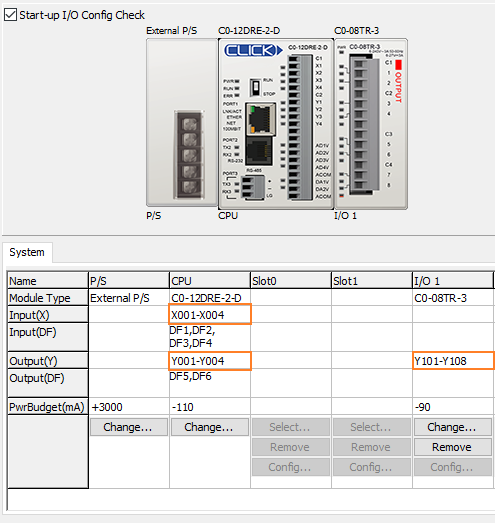
\includegraphics[width = 0.5\textwidth]{2_images/plcConfig.png}
            \caption{A snippet of the `System Configuration' window of the PLC showing onboard I/O address.}
            \label{fig:plcConfig}
        \end{figure}
        
        The reason that all \acrshort{io} is not exclusively "onboard", is due to long lead times of \acrshort{plc} expansion modules. We were lucky enough to get one digital output module which is responsible for the \acrshort{led} indicators on the front side of the Lolly Machine - three of which are a traffic light arrangement which show the Lolly Machine Status. A conscious decision was made to connect the status indicators directly to the \acrshort{plc} as in the event of a communications failure, there is the potential for the remote \acrshort{io} to fail whereas the onboard will not. 

        \begin{figure}[H]
            \centering
            
\includegraphics[width = 0.3\textwidth]{2_images/smile.png}
            \caption{The Click PLC and expansion digital output module.}
            \label{fig:plcIO}
            \HD{Picture of PLC with terminations}
        \end{figure}
    
    \subsection{Modbus I/O}
        Modbus \acrshort{io}, as the name suggests, are \acrshort{io} that are mapped to and from Modbus devices. As the \acrshort{plc} is a Client-Server device, there are two methods that must be discussed in regards to Modbus \acrshort{io} communication.

        \subsubsection{Server}
            The Modbus Server part of the \acrshort{plc} is accessible by Modbus Client devices. In the case of this project, these are the various control sources (\acrshort{hmi}s). Every variable within the \acrshort{plc} has an equivalent Modbus address which can be found within the `Address Picker' on the `Home' tab as illustrated by Figure \ref{fig:modbusAdd}. Next to the Modbus Addresses, are the function codes (see Table \ref{table:modbusFunctions}) that can be used to access the variable. There is no additional configuration that needs to be done to setup the the \acrshort{plc} as a Modbus Server device. 
            
        \begin{figure}[H]
            \centering
            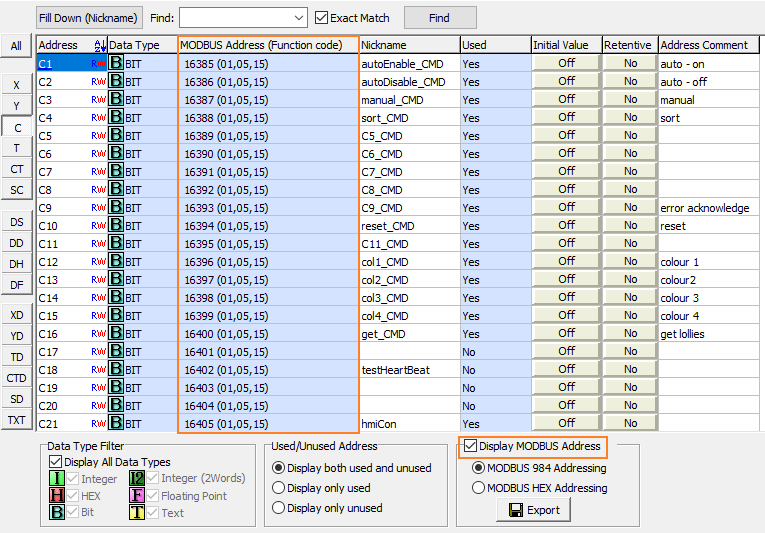
\includegraphics[width = 0.6\textwidth]{2_images/modbusAdd}
            \caption{Modbus Server addresses of the PLC.}
            \label{fig:modbusAdd}
        \end{figure}
        
            NOTE: Modbus address indexing can vary from device as some manufactures start from 0 while the others at 1. 
            
        \subsubsection{Client}
            The \acrshort{plc} Modbus Client is used to access the remote \acrshort{io} ADAM modules. Internal \acrshort{plc} addresses are linked Server Modbus address of the ADAM modules through the use of receive and send functions within the \acrshort{plc}. Figure \ref{fig:plcModbusClient} shows the send and receive functions for DAQ-03. The receive function (top) is reading 8 bits of data (8 addresses) with a starting Modbus address of 01 and mapping then to internal Boolean variables, C232 to C240. The send function (middle), is writing to 7 Modbus address on DAQ-03, from 17 to 24 - these are driven by internal variables C240 to C247.

            A maximum of one communication function can be executed per \acrshort{plc} cycle. A counter is used to alternate between each communication function as illustrated in Figure \ref{fig:plcModbusClient} (bottom function).

        \begin{figure}[H]
            \centering
            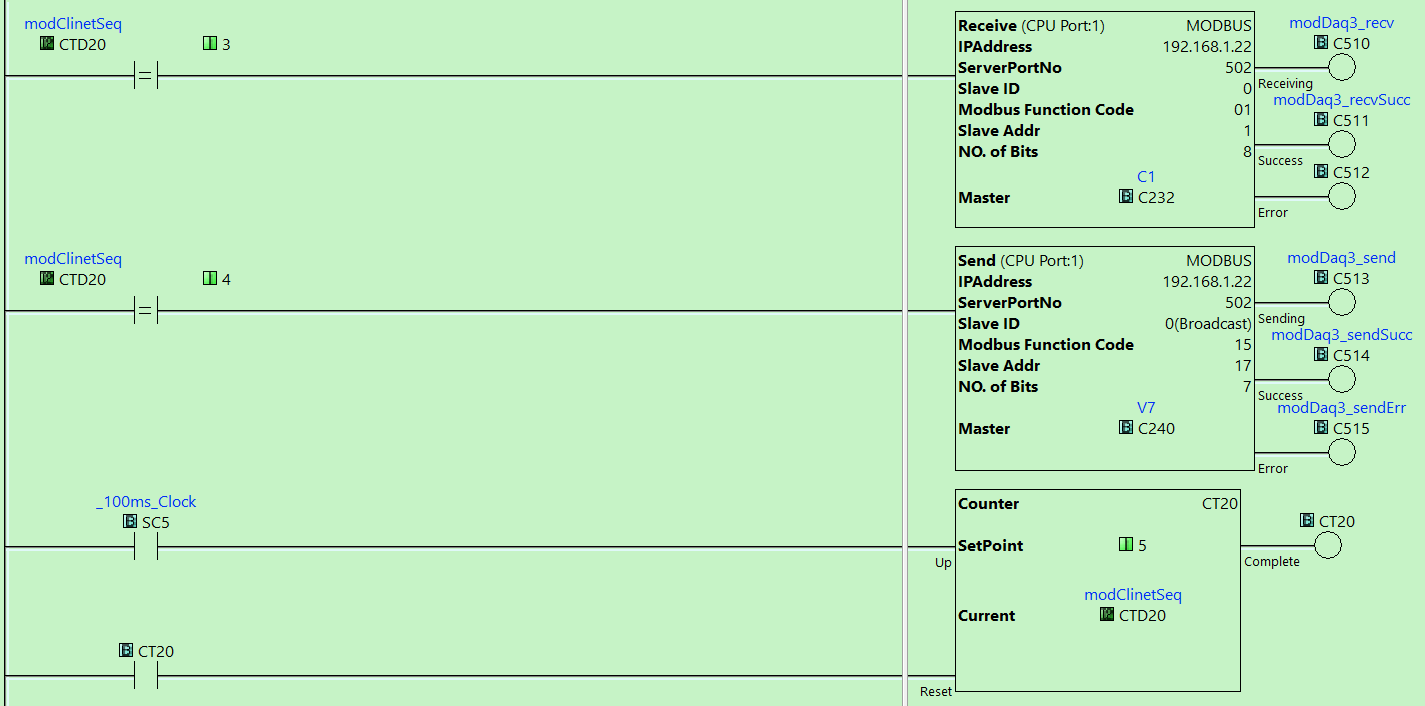
\includegraphics[width = 0.6\textwidth]{2_images/plcModbusClient}
            \caption{PLC Modbus Client send and receive functions within LL code.}
            \label{fig:plcModbusClient}
        \end{figure}
            
    \subsection{Input Mapping} \label{sec:input}
        Input mapping is almost exclusively concerned with virtual inputs from \acrshort{hmi} devices and can be found within the input subroutine program. The purpose of this portion of code is to define some logic that dictates which control source the \acrshort{plc} is taking instructions from. Figure \ref{fig:inputMapping}, for example, shows the three variables linked to each of the potential control sources (C301 - Siemens \acrshort{hmi}, C341 - LabVIEW application on \acrshort{ews} and C381 - Raspberry Pi) for the auto enable command - C1. Three internal variables (C21 Siemens \acrshort{hmi}, C22 - LabVIEW application on \acrshort{ews} and C23 Raspberry Pi) dictate which control source the \acrshort{plc} is currently taking instruction from. So,for C1 to be True, the \acrshort{plc} bust be taking instruction from the correct control source and the virtual output form the same control source must be true. After this is archived, \acrshort{no} contacts linked with C1 can be easily used wherever necessary within the program. 

        Without this input logic, the \acrshort{plc} will attempt to receive instruction from all three control sources at once.
        
        \begin{figure}[H]
            \centering
            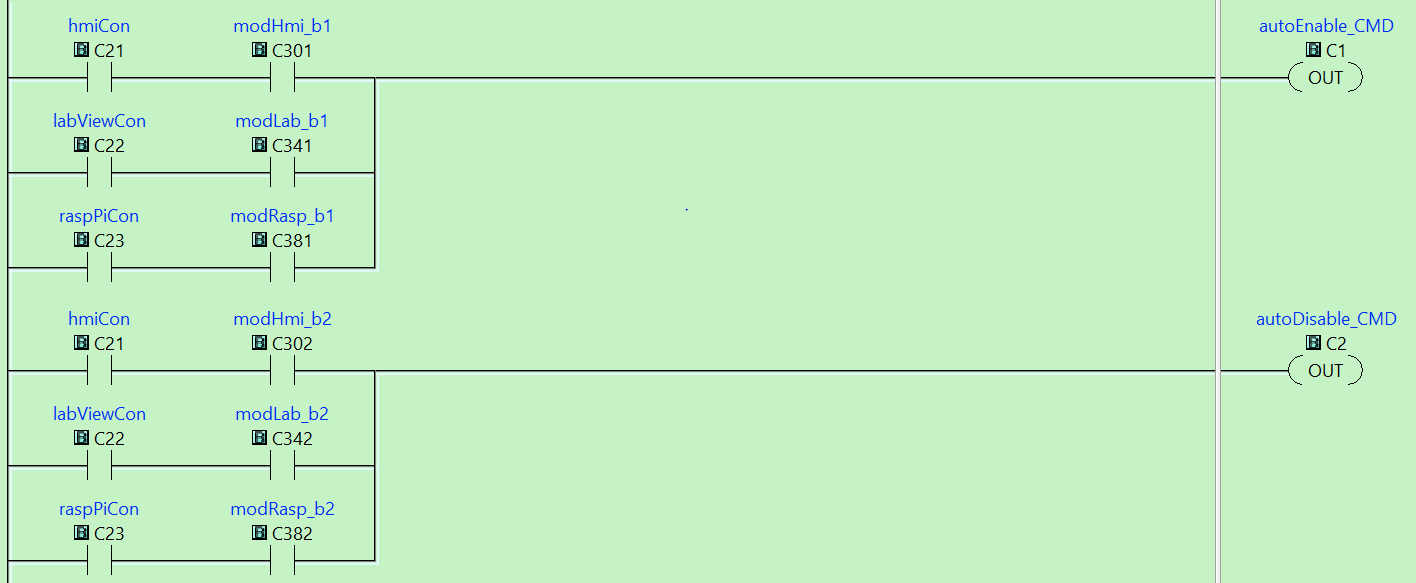
\includegraphics[width = 0.6\textwidth]{2_images/inputMapping}
            \caption{Input mapping from control sources.}
            \label{fig:inputMapping}
        \end{figure}
        
    \subsection{Output Mapping} \label{sec:output}


\section{Machine Design and Implementation}
    The overall structure of the \acrshort{plc} code has been written in a modular style where program functions are split into separate subroutines. Subroutine Programs are called from the Main Program as illustrated in Figure \ref{fig:plcMainAuto}. The Main Program is designed to be simple and easy to read. The only logic that exists within the Main Program is overall state machine which allows for the machine to be in one of three modes: Automatic, Manual or Alarm. \HD{Appendix for the PLC program.}

        \begin{figure}[H]
            \centering
            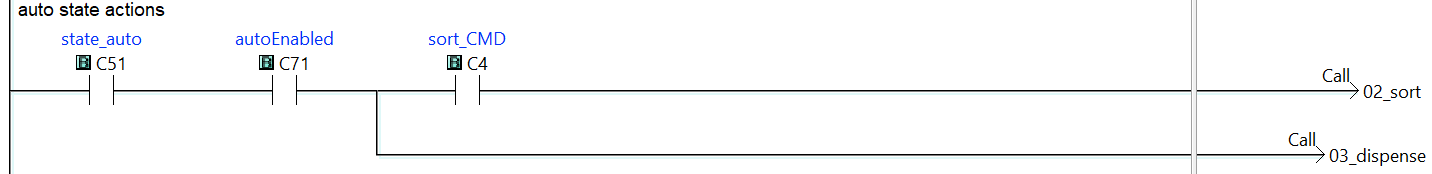
\includegraphics[width = 0.9\textwidth]{2_images/plcMainAuto}
            \caption{Snippet of PLC code showing where sort and dispense Subroutine Programs are called from the Main Program}
            \label{fig:plcMainAuto}
        \end{figure}
    The Main Program is also responsible for calling six other Subroutines Programs. This is achieved by connecting   ``\_Always\_ON'' \acrshort{no} contacts with each Subroutine Program.
    
    \subsection{Main Modes}
    A simplified version of State Machine Design has been implemented for the the Structure the Main Program. A graphical representation of the program can be seen in Figure \ref{fig:mainStateMachine}. The machine will swap between Manual and Automatic Mode as a function of the internal \acrshort{plc} variable C3. When an an Alarm exists within the machine the system will go into `Alarm Mode' regardless of whether the machine is in Manual or Automatic. 
    
        \begin{figure}[H]
            \centering
            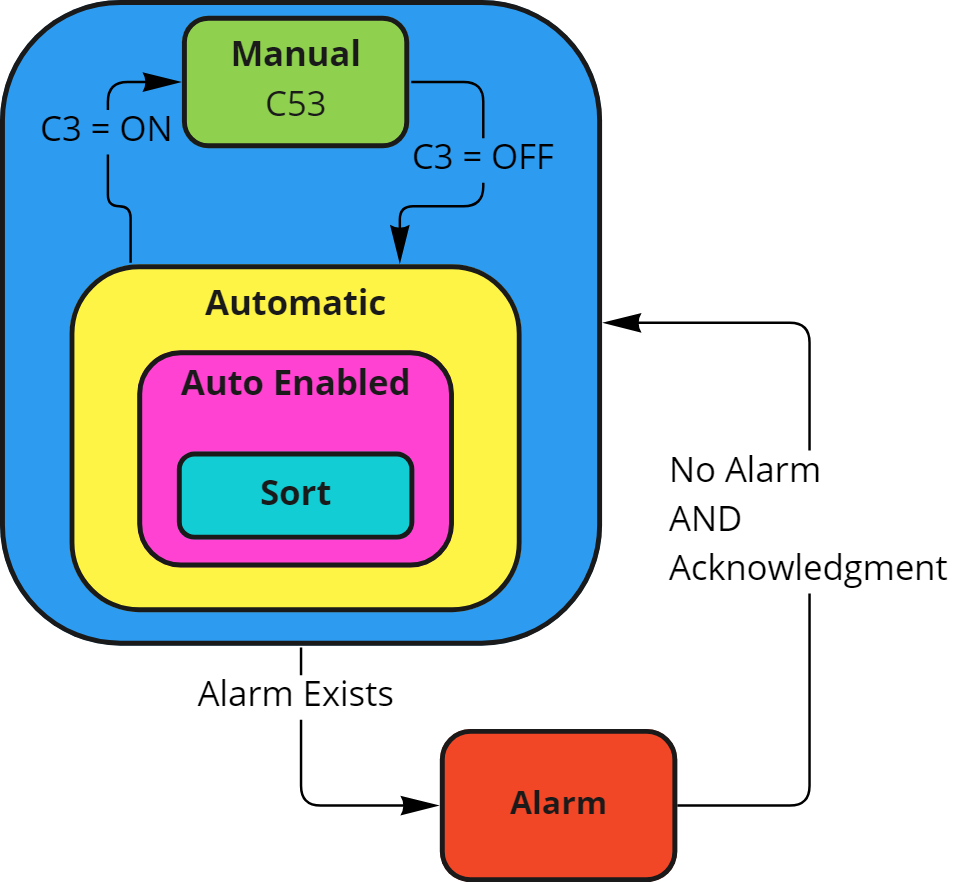
\includegraphics[width = 0.4\textwidth]{2_images/mainStateMachine}
            \caption{State Machine Design for the Main Program.}
            \label{fig:mainStateMachine}
        \end{figure}
    
        \subsubsection{Automatic}
            When C3 is off and the machine is not in an Alarm state, the machine will be in automatic mode. For the system to function in automatic mode, it must be enabled.  Once enabled, subroutine program `Dispense' is called. The `Sort' Subroutine is called when automatic mode is enabled and C4 is ON. The reason that these two subroutines are not called at the same time is to allow the machine to dispense while it is not sorting. 
            When the machine is in automatic mode, the green \acrshort{led} status indicator will flash when it is ready and will go solid once enabled.

        \subsubsection{Manual}
            When C3 is on and the machine is not in an alarm state, the machine will be in manual mode. While in manual mode, control valves can be manipulated via the connected control source. The logic that drives the manual control is detailed in Section \ref{sec:output}.
            When the machine is in manual mode, the amber \acrshort{led} status indicator will be on. 

        \subsubsection{Alarm}
            When an alarm is present, the machine will go into alarm mode. While in Alarm mode, the machine will be inoperable and outputs will go back to their default position. When the machine is in alarm mode, the red \acrshort{led} status indicator will be on.

    \subsection{Dispensing}
        Dispensing is a function of the lolly machine which is possible when the machine is enabled in automatic mode. While in this mode, the machine is constantly waiting for an input from the user to so that it knows which colour/s of lolly to dispense. Once the user has finished selecting the their desired colours, the user presses the get button and the machine will dispense the lollies. This is completed through general logic and can be found in appendix \HD{Appendix Number for the Ladder Logic Printout goes here}.
        \HD{Could add more detail here...}
        
    \subsection{Sort}
        The sorting subroutine is the most complex piece of code within the controller and has been written exclusively in state machine design. Rather than explain how this part of the program works, an illustration of the design is shown in Figure \ref{fig:sortStateMachine} which does a terrific job of showing all possible states and transitions. 

        \begin{figure}[H]
            \centering
            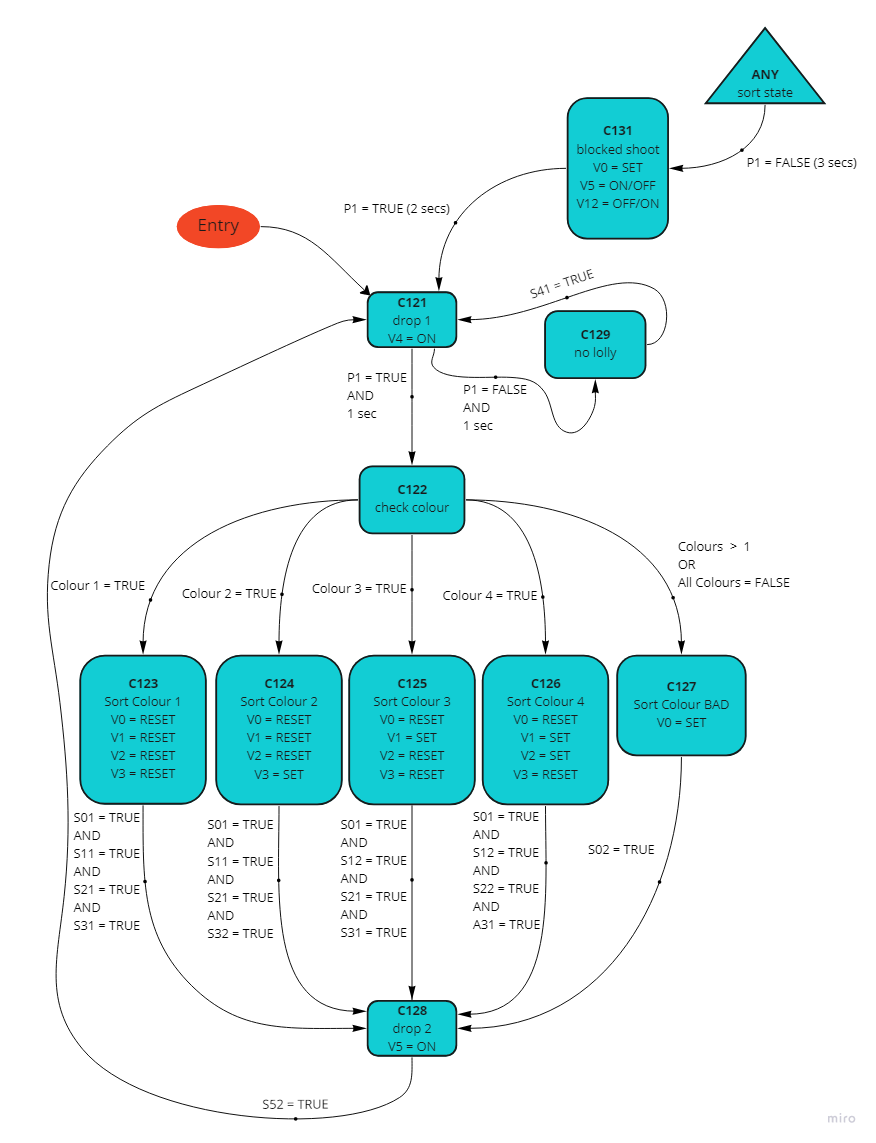
\includegraphics[width = 0.6\textwidth]{2_images/sortStateMachine}
            \caption{State machine design for the sorting program.}
            \label{fig:sortStateMachine}
        \end{figure}
        
    \subsection{Alarm Mode}



\section{Special Functions}

    \subsection{Automatic Shoot Unblock}

    \subsection{Automatic Control Source Recovery}

    \subsection{Valve FTO/ FTC} \label{sec:valveFtoFtc}

    